\documentclass{article}
\usepackage[normalem]{ulem}
\usepackage{fixltx2e}
\usepackage{color}
\usepackage[hidelinks]{hyperref}
\usepackage{graphicx}
\usepackage[top=2cm,bottom=2cm,left=3cm,right=3cm]{geometry}
\usepackage{multicol}
\usepackage{float}


\begin{document}
    \section{Literature Review}
	\subsection{The History of Robotic Control}
	Many different techniques and approaches for robotic control have been developed (Arkin, 1998). The robotic control system is, in fact, a continuous spectrum that ranges from purely deliberative reasoning at one extreme to purely reactive control at the other, with the myriad existing architectures fitting somewhere on the spectrum.
	
%	\begin{figure}[h!]
%	\centering
%	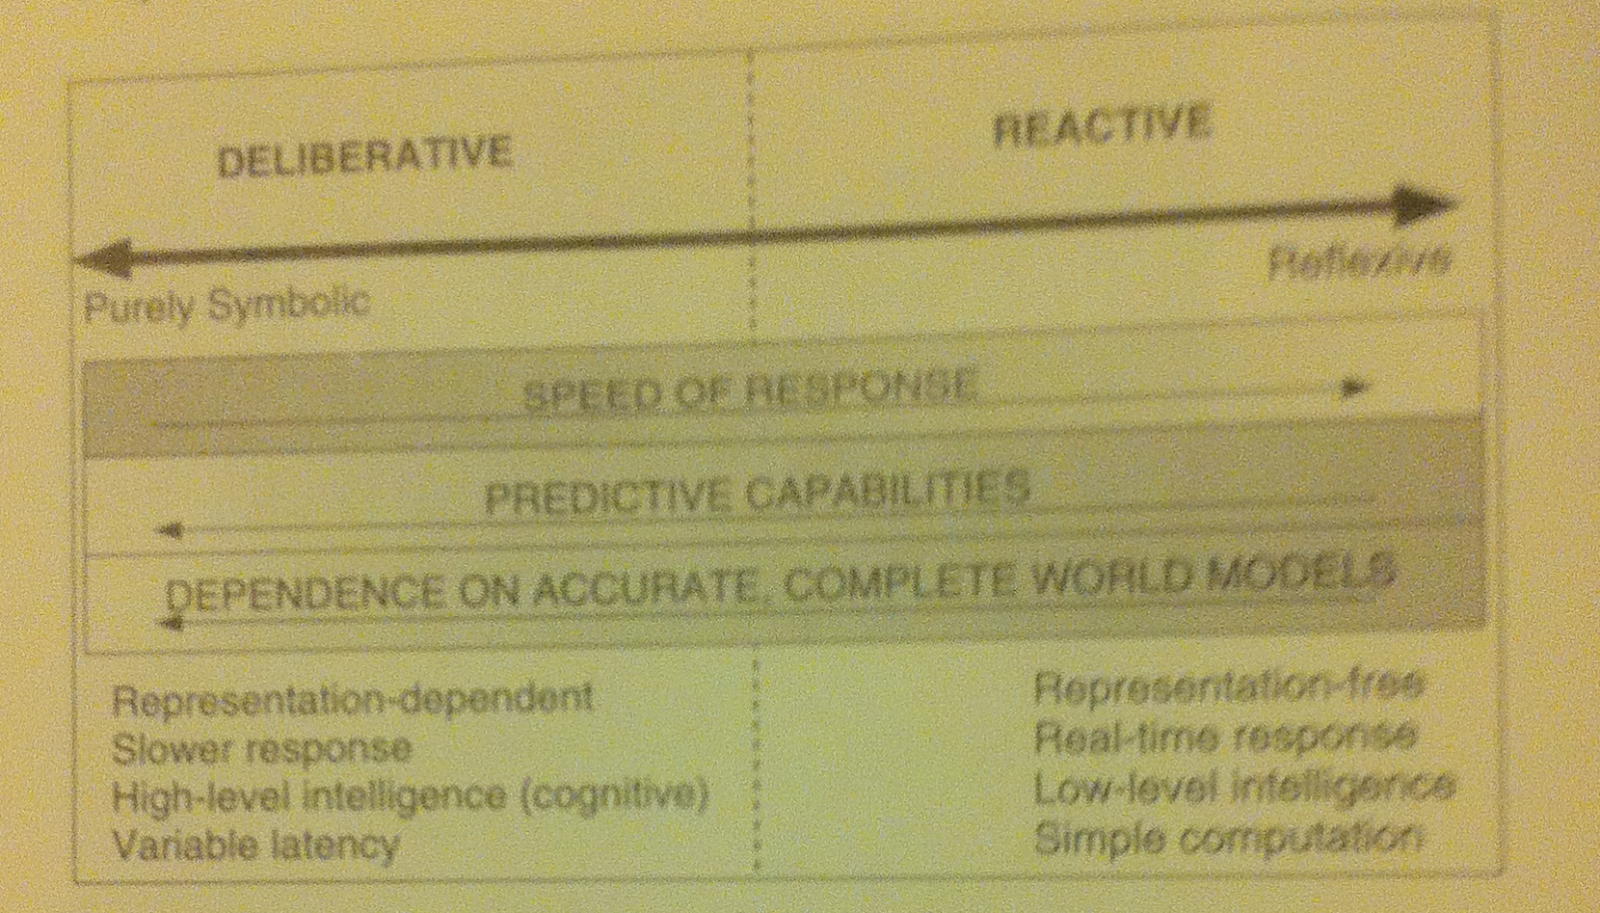
\includegraphics[width=0.8\linewidth]{LiteratureReview1}
%	\caption{Robot Control System Spectrum (Arkin, 1998)}
%	\end{figure}

	\subsubsection{Hierarchical Paradigm}
	The foremost paradigm of robotic control, the deliberative/hierarchical paradigm, focuses primarily on the planning stage of the behavioural cycle. Robots developed with a hierarchical architecture are essentially reflex agents [3], selecting actions from rule matches on the current ‘perceptions’ from sensory input. This approach typically employs a top-down view to design; an end-goal is realised and a sequence of modules are developed. These modules work to read values from the sensors available to gauge the proximate environment (perception), devise strategies to perform the desired behaviours given said perception (cognition), and then compose the signals that control the actuators to execute these behaviours to achieve the end goal (action).

	\begin{figure}[h!]
	\centering
	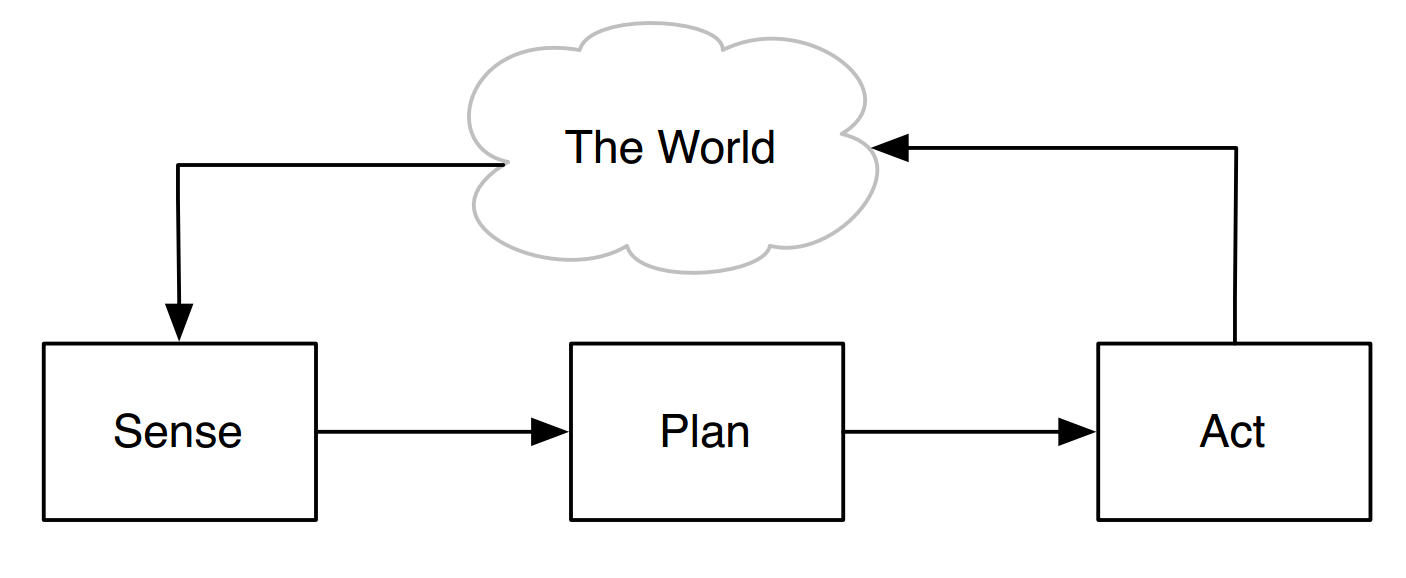
\includegraphics[width=0.8\linewidth]{LiteratureReview2}
	\caption{The typical structure of the hierarchical system of robot control}
	\end{figure}
	
	\subsubsection{Reactive Paradigm}
	The initial dominance enjoyed by the hierarchical paradigm was largely a result of the sphere of influence traditional Artificial Intelligence (AI) exerted over the sub-discipline of Robotics. The prevailing zeitgeist in AI at the time was the notion that knowledge, and knowledge representation, are central to intelligence [1]. Reactive control was born out of a shift against these traditions. Stellar to the reactive paradigm is the idea that the world is fundamentally unknown and changing, and that explicit symbolic representations of the world are simply unattainable. Arkin (1998, p. 24) describes reactive control as ‘a technique for tightly coupling perception and action, typically in the context of motor behaviours, to produce timely and robotic response in dynamic and unstructured worlds’ [1].

The highlights of the reactive paradigm include its basic building block - a behavior (a direct mapping of sensory inputs to the corresponding motor actions) and the removal of the planning stage from the Sense-Plan-Act triad [1]. In reactive systems, complex behaviours emerge as a consequence of the interaction of many smaller, individual behaviours, all working towards a global maxima (known as emergent behaviour). These behaviours can occur sequentially or concurrently, and each sensor is mapped to its own behaviour: essentially a stimulus/response pair. The set of behaviours to be executed are determined by the Robot’s immediate environmental context and as a result of the modularity of the behaviours, reactive systems are inherently modular from a software development perspective.

	\subsubsection{Behaviour-Based Robotics}
	The advent of the reactive paradigm also coincided with the birth of behaviour-based robotics. The behaviour based approach draws inspiration towards robot control from the disciplines of neuroscience, psychology and ethology (the science of animal behaviour), and to fully appreciate behavior-based robotics some background in biological behaviour is necessary.

Biological behaviors have been studied in three broad categories: reflexive behaviors, reactive behaviors and conscious behaviors [14]. Reflexive behaviors are direct stimulus-response mappings in which the response to a particular sensory input is directly wired with a response and carried out without any cognitive involvement; an example in humans being the kneejerk reaction to touching a hot plate. The second category concerns behaviors that are learned over time, such as learning to ride a bicycle or learning to walk in early childhood. Every other behavior that requires conscious thought throughout the time of the action is categorized as conscious behavior. 

Behaviour-based robotics is principally concerned with reflexive behaviours, which in robotics nomenclature are labelled ‘reactive’. One of the pioneering behavioural-based architectures is subsumption, a reactive approach presented by Rodney Brooks in 1987 [15]. Subsumption builds on layers of competencies (or simply, a collection of behaviors to achieve a specific task) that are vertically arranged in the order of their sophistication. Basic behaviors, such as collision avoidance, are aligned in the lowest layer, while more cognitive behaviors, such as path mapping, are aligned in the higher levels [14]. The higher layers have the ability to inhibit or suppress the behaviors of the lower layers, hence the name subsumption. The layers of behaviour are designed to be ignorant of one another; each layer executes a dedicated behavior and this avoids the need for them to know the complete scenario they are trying to solve.

	\subsubsection{Hybrid Paradigm}
	Whilst the reactive paradigm emerged as the solution for the rigidities put forth by the hierarchical paradigm, the need for planning in more complex tasks began to show over time. Hence, roboticists looked into new ways of combining a planning process with reactive behaviors. Thus, a new breed of architecture was born, the ‘Hybrid Deliberative/Reactive paradigm’. 

The hybrid paradigm altered the Sense-Plan-Act trilogy by allowing the Plan stage to be executed separately from the Sense-Act sequence. Arkin (1998) mentions three ways in which planning and reaction can be integrated [1]:
\begin{enumerate}
\item Hierarchical integration of planning and reaction - The planning and reaction layer are aligned vertically with the planning layer providing the information on which the reaction layer acts.

\item Planning to guide reaction - Planning configures and sets parameters for the reaction control system. Execution occurs solely under the reactive system's auspices, with planning occurring both prior to and concurrent with execution.

\item Coupled planning-reaction - Planning and reaction are concurrent activities, each guiding the other.
\end{enumerate}

A 1995 workshop indicated that a multi-layered hybrid architecture comprising of a top-layer planning system and a lower level reactive system is the emerging architecture of choice in robot control design [1].

	\subsection{Localisation}
	Localisation, as applied to Robotics, is the difficult task for an autonomous robot to construct or use a map (or floor plan) and correctly position itself within it. There are several methods and technologies available to the end of achieving localisation including, but not limited to, GPS, odometry (dead reckoning\footnote{The process of calculating one's current position by using a previously determined position, or fix, and advancing that position based upon known or estimated speeds over elapsed time and course; for example using the number of wheel revolutions of the robot.}) and laser and sonar. In each approach however, improvements in accuracy come at the cost of increasingly expensive hardware and  additional processing power. 

A robot has two types of information sources in regards to localization: the idiothetic and the allothetic, and most biologically-inspired models for robots use a combination of both [5]. Tracking the number of wheel revolutions of the Robot is an idiothetic source, and whilst it can give the absolute position of the Robot, it can become subject to cumulative error which grows rapidly. Allothetic sources, by contrast, are the sensors of the robot (such as laser and sonar). The problem with allothetic sources  is "perceptual aliasing", which is where two different places can be perceived as the same. In an office building, for example, it may be impossible to correctly localise from sensor information alone if all corridors are identical (and thus providing identical or near-identical sensory feedback).

The general localization problem has a number of increasingly difficult problem instances [6]. The first of these is ‘position tracking’ and in this problem the robot knows its initial position. With position tracking the goal of localization is to maintain knowledge of the robot’s position whilst it navigates through the environment.  Techniques that solve this problem are called tracking or local techniques [7]. 

The ‘wake-up robot’ or ‘global positioning’ problem is more difficult than the position tracking problem, since the robot does not know its initial position and instead has to localize itself from scratch. Thus, it needs to be able to deal with multiple ideas about its possible location. Methods that solve this problem are called global techniques [7]. 

An even harder problem to solve is the ‘kidnapped robot’ problem, wherein the robot  knows where it is localized but is transferred to another location without knowing. The robot thus has to detect that it has been kidnapped and then re-localize. Techniques that solve this problem can also be used to solve the wake-up robot problem, which can be considered a special instance of the kidnapped robot problem [7].

	\subsubsection{Markov Localisation}
	The localization problem can itself be described as a bayesian estimation problem: the robot has a belief about where it currently is and the problem consists of computing the probability density over the space of all possible locations. A bayesian framework for so doing is the Markov Localisation framework originally developed by Thrun et al [7]. The Markov framework assigns weights (a probability) to points on the map from sensory and odometry data and updates these as new data is received, forming a combined overall belief in the location of the robot. Markov Localisation techniques often assume the environment is static (the markovian assumption) [8]. This assumption postulates that the robot's location is the only state in the environment which systematically affects sensor readings. More formally, it states that the sensor measurements observed at time t are independent of all other measurements, given that the current state Lt of the world is known. In the case of localization in densely populated environments, this independence assumption is clearly violated when using a static model of the world. [8]

	\subsubsection{Kalman Filters}
	Another Bayesian localization algorithm is the Kalman Filter. Kalman Filters operate recursively on streams of noisy input data to produce a statistically optimal estimate of the underlying system state. The ‘state’ of a system refers to a vector, x, consisting of n variables describing some interesting properties of the system. An example of a state is the location of a robot, consisting of the x and y coordinates, and the orientation O, of a robot.

	Kalman-filter based techniques have proven to be robust and accurate for keeping track of a robot’s position [9,10]. Because of its concise representation (the mean and covariance matrix suffice to describe the entire density) it is also a particularly efficient algorithm [11]. However, in its pure form, the Kalman filter does not correctly handle non-linear or non-Gaussian motion and measurement models, is unable to recover from tracking failures, and can not deal with multi-modal densities as encountered during global localization. Whilst non-linearities, tracking failure and even multi-modal densities can be accommodated using non-optimal extensions of the Kalman filter, most of these difficulties stem from the the restricted Gaussian density assumption inherent in the Kalman filter [11].

	\subsubsection{Monte Carlo Localization}
	A final technique to discuss is the (Adaptive) Monte Carlo localization approach (as described by Dieter Fox),  which is included in the ROS Navigation framework [12]. This is also the localization approach we adopted for our Robot. The Monte Carlo approach is an technique to determine a Robot’s position and orientation (pose) using a particle filter,  wherein each particle represents a possible pose of the Robot. The rationale for using a  particle filter to solve the localization problem is clear. Unlike Kalman Filters, particle filters can approximate a wide variety of probability distributions, not just gaussian distributions. They are also computationally efficient, as they focus resources on regions in state space with high likelihood [13]. 

The basic principle of particle filters is having a perceptual model, p(zt | xt) that describes the likelihood of making the observation zt, given that the robot is at location xt, for each particle in the state space s. As new sensory and odometry readings are obtained, the model is updated by recursively replacing the particles using a method of probabilistic sampling [16].  

The ‘Adaptive’ extension to Monte Carlo Localization, developed by Dieter Fox, uses KLD-sampling to dynamically update the size of sample sets [17]. The key idea of the KLD-sampling method is to bound the approximation error introduced by the sample-based representation of the particle filter, and is so named because the approximation error is measured by the Kullback-Leibler distance\footnote{A measure of how different two probability distributions (over the same event space) are [18].} [17]. During the initial global localization, a robot may be highly uncertain of its pose, and thus a large number of samples required to accurately represent its belief. Once it has positioned itself, however, only a small sample set is required for the easier localization problem of position tracking [16]. KLD-sampling adapts the number of samples during the localization process, choosing large sample sets during global localization and small sample sets for position tracking [16].

	\subsection{Motion Planning}
	The basic motion planning problem in robotics is the challenge of moving a robot from one position to another whilst avoiding obstacles. It is also referred to as the ‘navigation problem’ or ‘piano mover’s problem’ and many mobile robot navigation problems can be expressed as instances of the basic motion planning problem [19]. There exist a large number of techniques to solve the basic motion planning problem, however not all of them solve the problem in its full generality [19]. 

In motion planning, a configuration describes the pose of the robot, and the configuration space C is the set of all possible configurations. Every obstacle in the configuration space can be mapped to a subset of C, C\textsubscript{obstacle}. The complement of C\textsubscript{obstacle} is the ‘free’ space and labelled C\textsubscript{free}. The basic motion planning problem is solved by creating a path between two configurations, qinit and q\textsubscript{goal}, through a connected region of C\textsubscript{free} [19].

The first extension to the basic planning problem, and the one that concerns our solution, is the presence of moving obstacles. In this instance, the problem can not be solved by simply constructing a geometric path through C\textsubscript{free}[19]. Rather, a continuous function of time must be calculated specifying the robots configuration at each instant [19]. This is achieved by adding one dimension representing time, C\textsubscript{T}, to the robot’s configuration space [19].

Grid-Based searches are one technique for solving motion planning problems, and the ROS navigation stack adopts a grid-based search algorithm [20]. Grid-based approaches overlay a grid on the configuration space, and assume each configuration is identified with a grid point. At each grid point, the robot is allowed to move to adjacent grid points as long as the line between them is completely contained within C\textsubscript{free}.

The specific technique the ROS Navigation stack uses is a grid-based costmap, wherein each cell in the map has one of three states: occupied, free, or unknown, and is assigned a cost (hence the term costmap). Occupied cells are assigned a lethal (infinite) cost, meaning that no part of the robot can step inside that cell. The global planner is given the obstacle and cost information contained in the Costmap, information from the robot’s localization system, and a goal in the world. From these, it creates a high-level plan for the robot to follow to reach the goal location using the lowest cost route. For speed of processing, the navigation uses an A* algorithm [27]. As the PR2 navigation system (the ROS Navigation system) successfully completed 26.2 miles of autonomous navigation in an office environment, without human intervention [27], it is provenly suitable to solve the Call a Meeting challenge.

\subsection{Person Detection}
In recent years, the social aspect of service robots has made it clear that they are not only expected to navigate within their environment but also to interact with people so as to provide useful services.  Thus, they need to be aware of the presence and position of the people with whom they are interacting [28]. This is, however, a very challenging task; people’s behaviour is often completely unpredictable [28]. Critical to the success of this task is the ability of the robot to identify and interact with people, and, thus, a robust method of so doing is required.

The most common devices used for people identification and tracking are laser sensors and cameras [29]. The solution we adopted is laser-based leg detection system that uses the front-mounted laser scanner and was taken from the thesis work of one of the module demonstrators, Marco Becerra, and is available (in Spanish) at [29].  Marco’s work is itself based on the work of Nicola Bellotto and Huosheng Hu, available at [28].

The basic premise of the detection algorithm is to identify typical patterns (relative to particular leg postures) that, in most of the cases, are well distinguishable from the other objects in the environment. These patterns correspond to the following three typical situations: two legs apart (LA), forward straddle (FS), and two legs together or (SL). The first pattern is usually very common in case the person is standing in front of the robot. The second, however, is most likely to happen when the person is walking. The last pattern covers most of the remaining possible postures. The results of the laser scan are preprocessed into a string pattern, and then checked for likeness to any of the typical leg patterns (subject to standard human dimensions - e.g. a leg cannot be 10 meters wide) through regular expression matching.
\end{document}